\section{Worksheet 4}
\subsection{Triangle Meshes}
We want to be able to render arbitrary surface. One way to do this is by using triangle meshes. We now load the Cornell box along with it's blocks instead of the default scene. The preview can be seen from figure \ref{fig:cornell_base_rendering}
\begin{figure}[H]
	\centering
	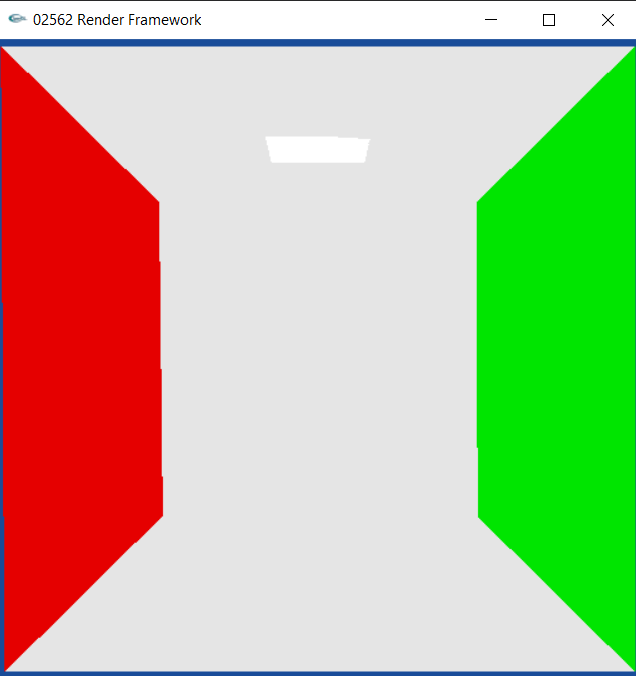
\includegraphics[scale=\imagescale]{images/worksheet_4/part_1}
	\caption{Cornell box base rendering}
	\label{fig:cornell_base_rendering}
\end{figure}
To implement ray tracing we have to implement the intersection function for the triangle meshes. This function is very similar to the intersection function for the triangles that we implemented on worksheet 1. The rendering obtained with ray tracing and base colours can be seen in figure \ref{fig:cornell_base_ray_tracing}.
\begin{lstlisting}
bool TriMesh::intersect(const Ray& r, HitInfo& hit, unsigned int prim_idx) const
{
	const uint3& face = geometry.face(prim_idx);
	const uint3& in_face = normals.face(prim_idx);
	float3 v0 = geometry.vertex(face.x);
	float3 v1 = geometry.vertex(face.y);
	float3 v2 = geometry.vertex(face.z);
	float3 n;
	float t;
	float v;
	float w;
	bool has_hit = ::intersect_triangle(r, v0, v1, v2, n, t, v, w);
	float u = 1.0f - v - w;
	
	if (has_hit) {
		hit.has_hit = true;
		hit.dist = t;
		hit.geometric_normal = -normalize(n);
		hit.shading_normal = hit.geometric_normal;
		
		hit.material = &materials[mat_idx[prim_idx]];
		hit.position = r.origin + r.direction * hit.dist;
	}
	return has_hit;
}
\end{lstlisting}

\begin{figure}[H]
	\centering
	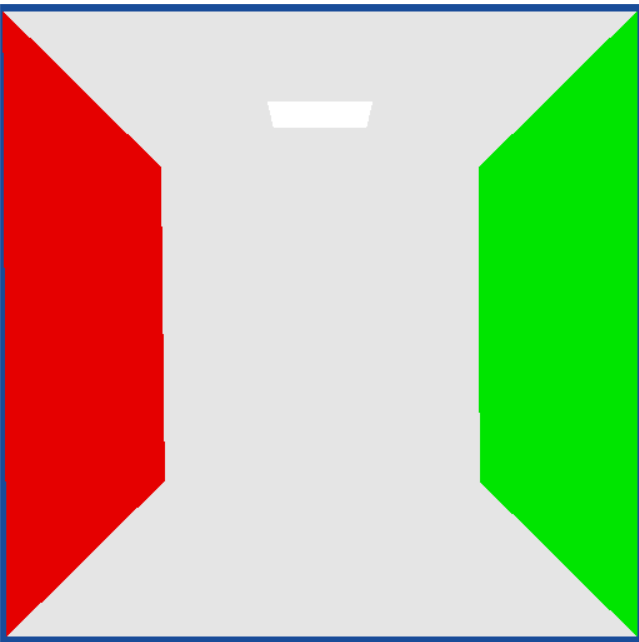
\includegraphics[scale=\imagescale]{images/worksheet_4/part_2}
	\caption{Cornell ray tracing base colour rendering}
	\label{fig:cornell_base_ray_tracing}
\end{figure}
The cornell box has an area light, to enable this source we have to implement the AreaLight::sample method.	
\begin{lstlisting}
bool AreaLight::sample(const float3& pos, float3& dir, float3& L) const
{
	const IndexedFaceSet& normals = mesh->normals;
	int n_faces = mesh->geometry.no_faces();
	float3 light_pos = mesh->compute_bbox().center();
	
	dir = light_pos - pos;
	float dir_norm = length(dir);
	dir = normalize(dir);
	
	float3 intensity = make_float3(0.0f);
	for (int i = 0; i < n_faces; i++) {
		uint3 face = mesh->geometry.face(i);
		float3 face_normal = normalize(normals.vertex(face.x) + normals.vertex(face.y) + normals.vertex(face.z));
		intensity = intensity + dot(-dir, face_normal) * get_emission(i) * mesh->face_areas[i];
	}
	
	float epsilon = 1e-4;
	float cutoff_distance = dir_norm - epsilon;
	Ray shadow_ray = Ray(pos, dir, 0, epsilon, dir_norm-epsilon);
	HitInfo hit_info = HitInfo();
	tracer->trace_to_any(shadow_ray, hit_info);
	
	if (!hit_info.has_hit) {
		L = intensity / (dir_norm * dir_norm);
	}
	return !hit_info.has_hit;
	
}
\end{lstlisting}

\begin{figure}[H]
	\centering
	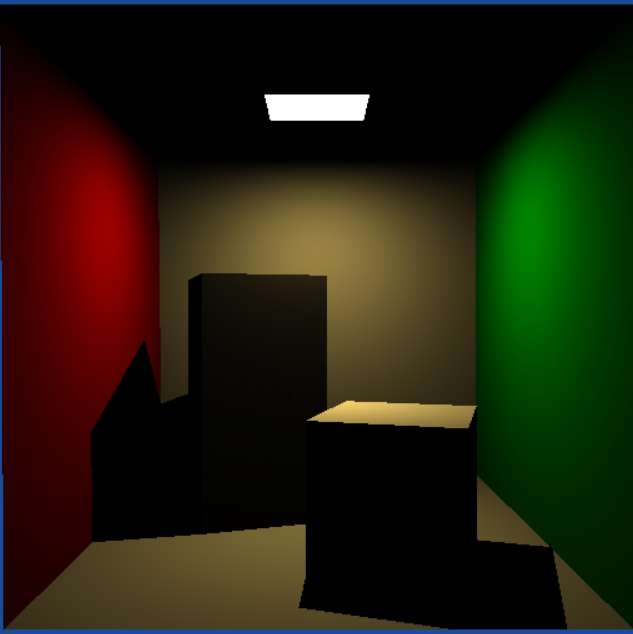
\includegraphics[scale=\imagescale]{images/worksheet_4/part3_after_rendering}
	\caption{Cornell Box with flat shading}
	\label{fig:cornell_lambertian_shading}
\end{figure}
We load now a different triangle mesh, the Utah teapot. The teapot is lit by a default directional light. To enable this source we have to implement then the function Directional::sample.
\begin{lstlisting}
bool Directional::sample(const float3& pos, float3& dir, float3& L) const
{
	dir = -light_dir;
	
	//Worksheet2 - point 1
	float epsilon = 1e-4;
	float cutoff_distance = RT_DEFAULT_MAX;
	
	Ray shadow_ray = Ray(pos, dir, 0, epsilon, RT_DEFAULT_MAX);
	HitInfo hit_info = HitInfo();
	
	tracer->trace_to_any(shadow_ray, hit_info);
	if (!hit_info.has_hit) {
		L = emission;
	}
	return !hit_info.has_hit;
}
\end{lstlisting}

\begin{figure}[H]
	\centering
	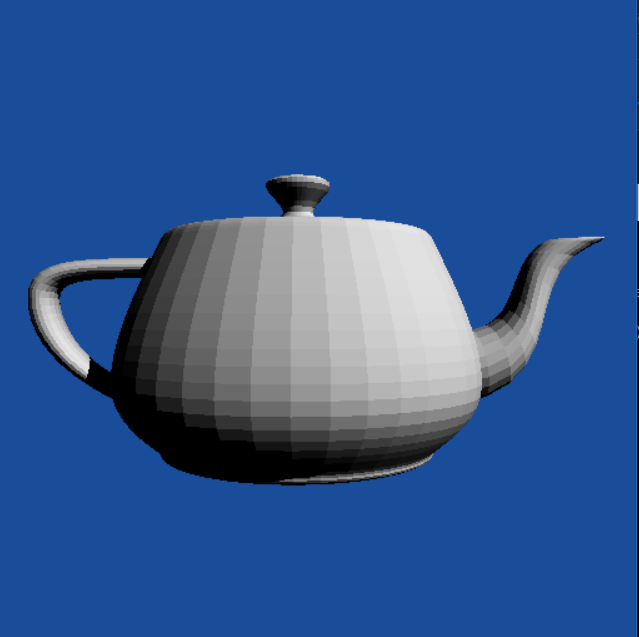
\includegraphics[scale=\imagescale]{images/worksheet_4/part4_after_rendering}
	\caption{Utah teapot with flat shading}
	\label{fig:utah_lambertian}
\end{figure}
As we can see from figure \ref{fig:utah_lambertian} the result looks pretty blocky. This can be solved by using interpolation of vertex normals. We have to appropiately modify the intersect function of the Triangle Mesh that we made before.
\begin{lstlisting}
bool TriMesh::intersect(const Ray& r, HitInfo& hit, unsigned int prim_idx) const
{
	const uint3& face = geometry.face(prim_idx);
	const uint3& in_face = normals.face(prim_idx);
	float3 v0 = geometry.vertex(face.x);
	float3 v1 = geometry.vertex(face.y);
	float3 v2 = geometry.vertex(face.z);
	
	
	float3 n;
	float t;
	float v;
	float w;
	bool has_hit = ::intersect_triangle(r, v0, v1, v2, n, t, v, w);
	float u = 1.0f - v - w;
	
	if (has_hit) {
		hit.has_hit = true;
		hit.dist = t;
		hit.geometric_normal = -normalize(n);
		if (has_normals()) {
			hit.shading_normal = normalize(u * normals.vertex(in_face.x) + v * normals.vertex(in_face.y) + w * normals.vertex(in_face.z));
		}
		else {
			hit.shading_normal = hit.geometric_normal;
		}
		hit.material = &materials[mat_idx[prim_idx]];
		hit.position = r.origin + r.direction * hit.dist;
	}
	return has_hit;
}
\end{lstlisting}

\begin{figure}[H]
	\centering
	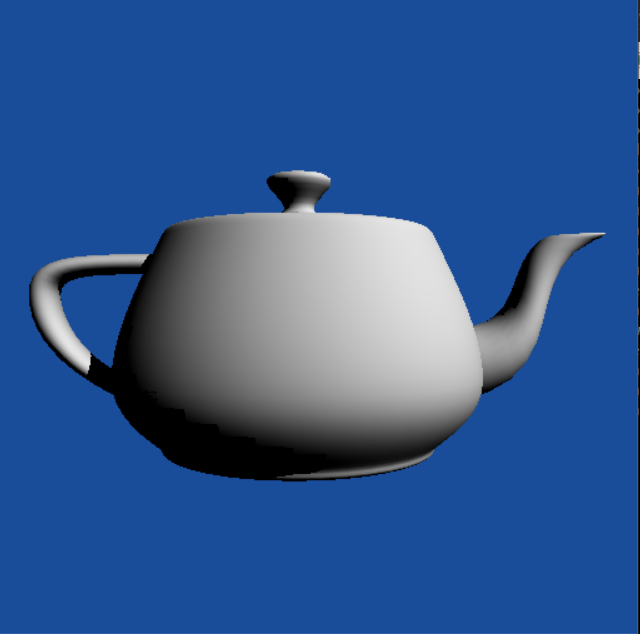
\includegraphics[scale=\imagescale]{images/worksheet_4/part_5}
	\caption{Utah teapot with interpolation between normals}
	\label{fig:utah_interpolation}
\end{figure}
As we can see from figure \ref{fig:utah_interpolation} the result looks much better now.
\subsection{Space Subdivision}
To make the renderings of our polygons much faster we need to use a more efficient data structure to check for intersections.\\
We do this by using the given implementation of the BSP data structure. The main idea behind BSP trees is the fact that hyperplanes subdivide the 3-dimensional space in two. We start in a situation where our tree is formed by a single node containing all of the primitive polygons of our objects in the scene, then we chose the polygon contained in the hyperplane which best subdivides the scene. Now we modify our tree such that the root of our tree becomes the polygon related to the hyperplane we selected before and that  the left and right sub-nodes contain all of the polygons on one side and the other of the selected hyperplane. We repeat this recursevely for both of the subnodes of the tree.


\begin{lstlisting}
bool BspTree::closest_hit(Ray& r, HitInfo& hit) const
{
	closest_plane(r, hit);
	intersect_min_max(r);
	intersect_node(r,hit,*root);
	return hit.has_hit;
}

bool BspTree::any_hit(Ray& r, HitInfo& hit) const
{
	any_plane(r, hit);
	intersect_min_max(r);
	intersect_node(r, hit, *root);
	return hit.has_hit;
}
\end{lstlisting}

\begin{table}[H]
	\centering
	\begin{tabular}{|l|l|l|l|}
		\hline
		\textbf{}                       & \textbf{Number of Triangles} & \textbf{Default} & \textbf{BSP Tree} \\ \hline
		\textbf{Stanford Bunny}         & 69451                        & 337.853          & 0.15              \\ \hline
		\textbf{Utah Teapot}            & 6320                         & 22.449s          & 0.279s            \\ \hline
		\textbf{Cornell Box and Blocks} & 24                           & 0.205            & 0.086s            \\ \hline
	\end{tabular}
	\caption{Time comparison between our default data structure and the BSP Tree}
	\label{table:time_comparisons}
\end{table}
From table \ref{table:time_comparisons} we can see that with our default data structure the time complexity seems to increase linearly with the number of triangles of the polygon.\\
On the other with the BSP data structures it doesn't seem to be a linear relation between the time complexity and the number of triangles since the utah teapot takes almost double the time of the stanford bunny despite the fact it has a number of trinagles which is ten times lower.
Despite this the rendering times drop substantially in all of the cases.